\section{Zavaró jel PD szabályozóval (Szorgalmi feladat)}

A levezetés \aref{sec:szorg-pi}. feladatéhoz analóg módon történik annyi különbséggel, hogy
$\fn{W}_\text{c}$ nem PI, hanem PD szabályzó.

\begin{figure}[H]
	\centering
	\begin{subfigure}{.49\textwidth}
		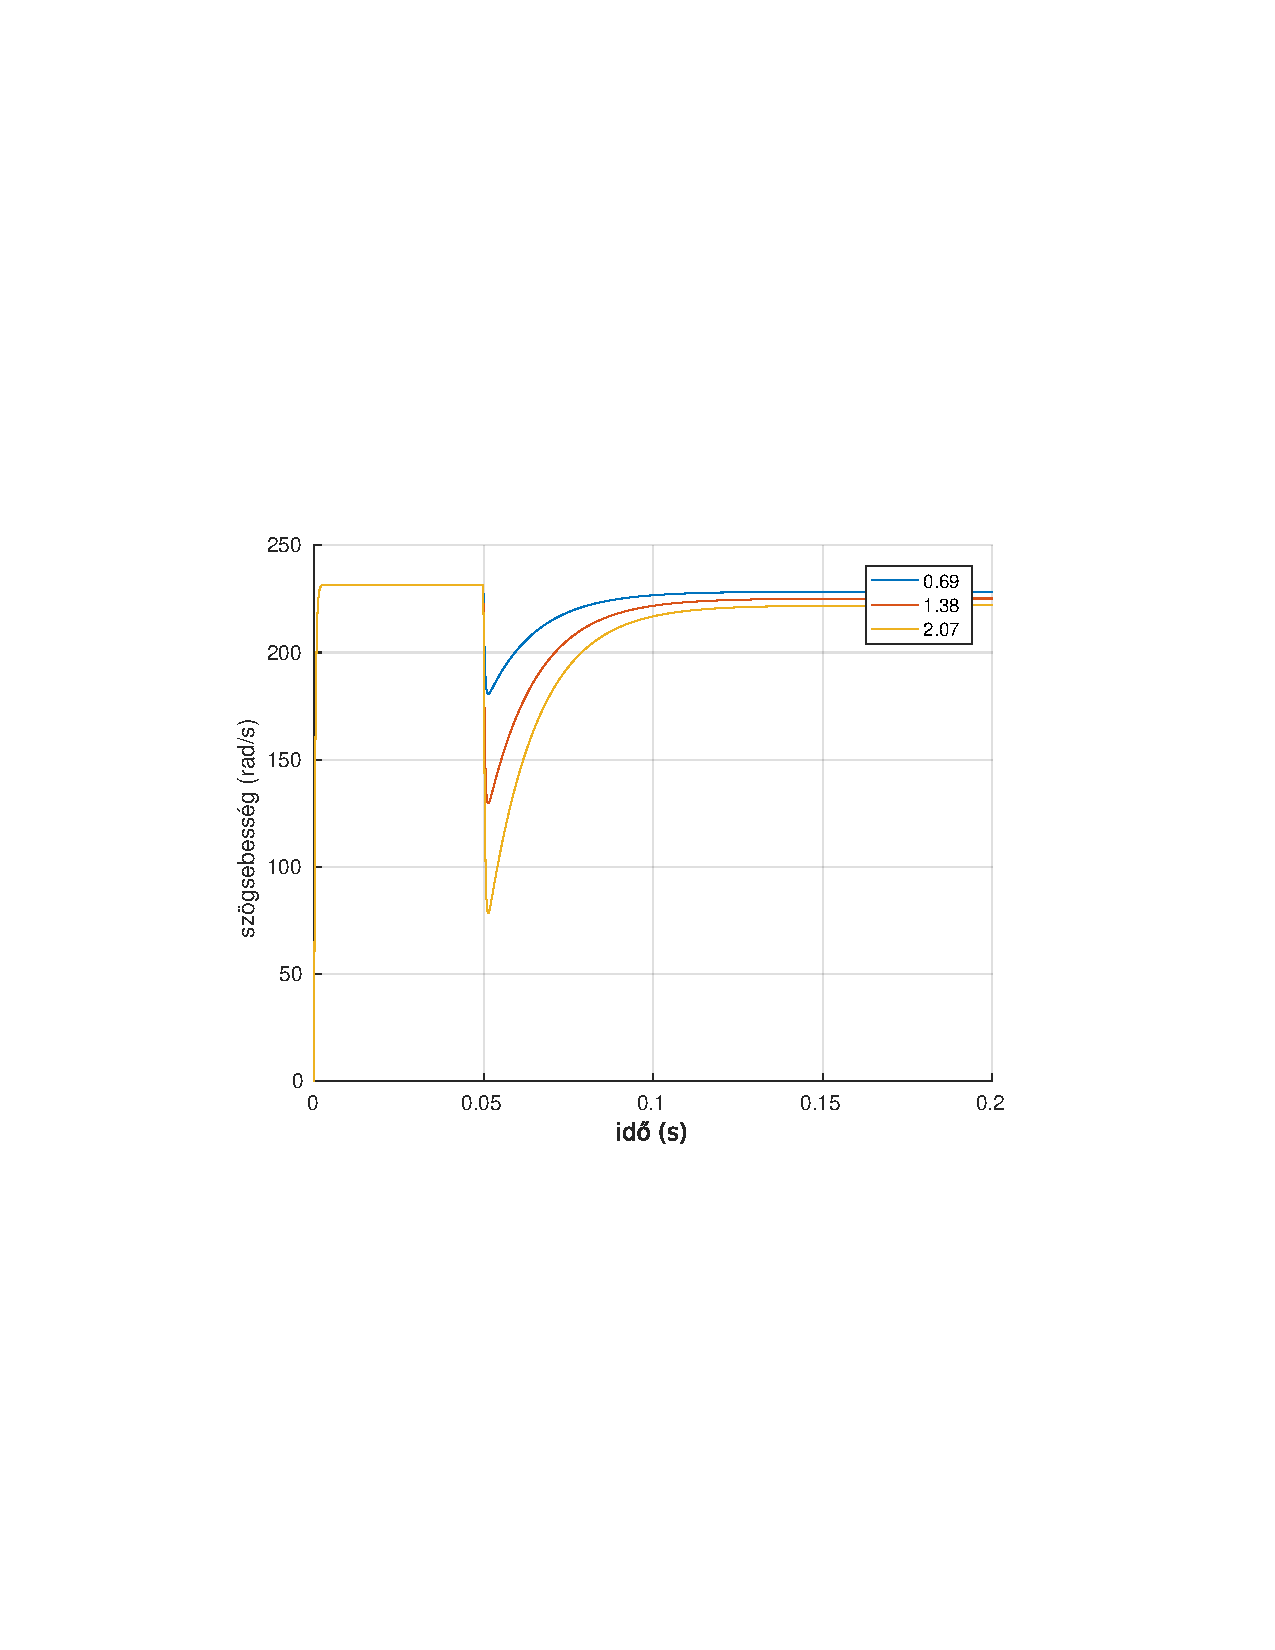
\includegraphics[width=\linewidth, trim=100 240 80 252, clip]{6-w}
		\caption{Szögsebesség válasz}
	\end{subfigure}
	\begin{subfigure}{.49\textwidth}
		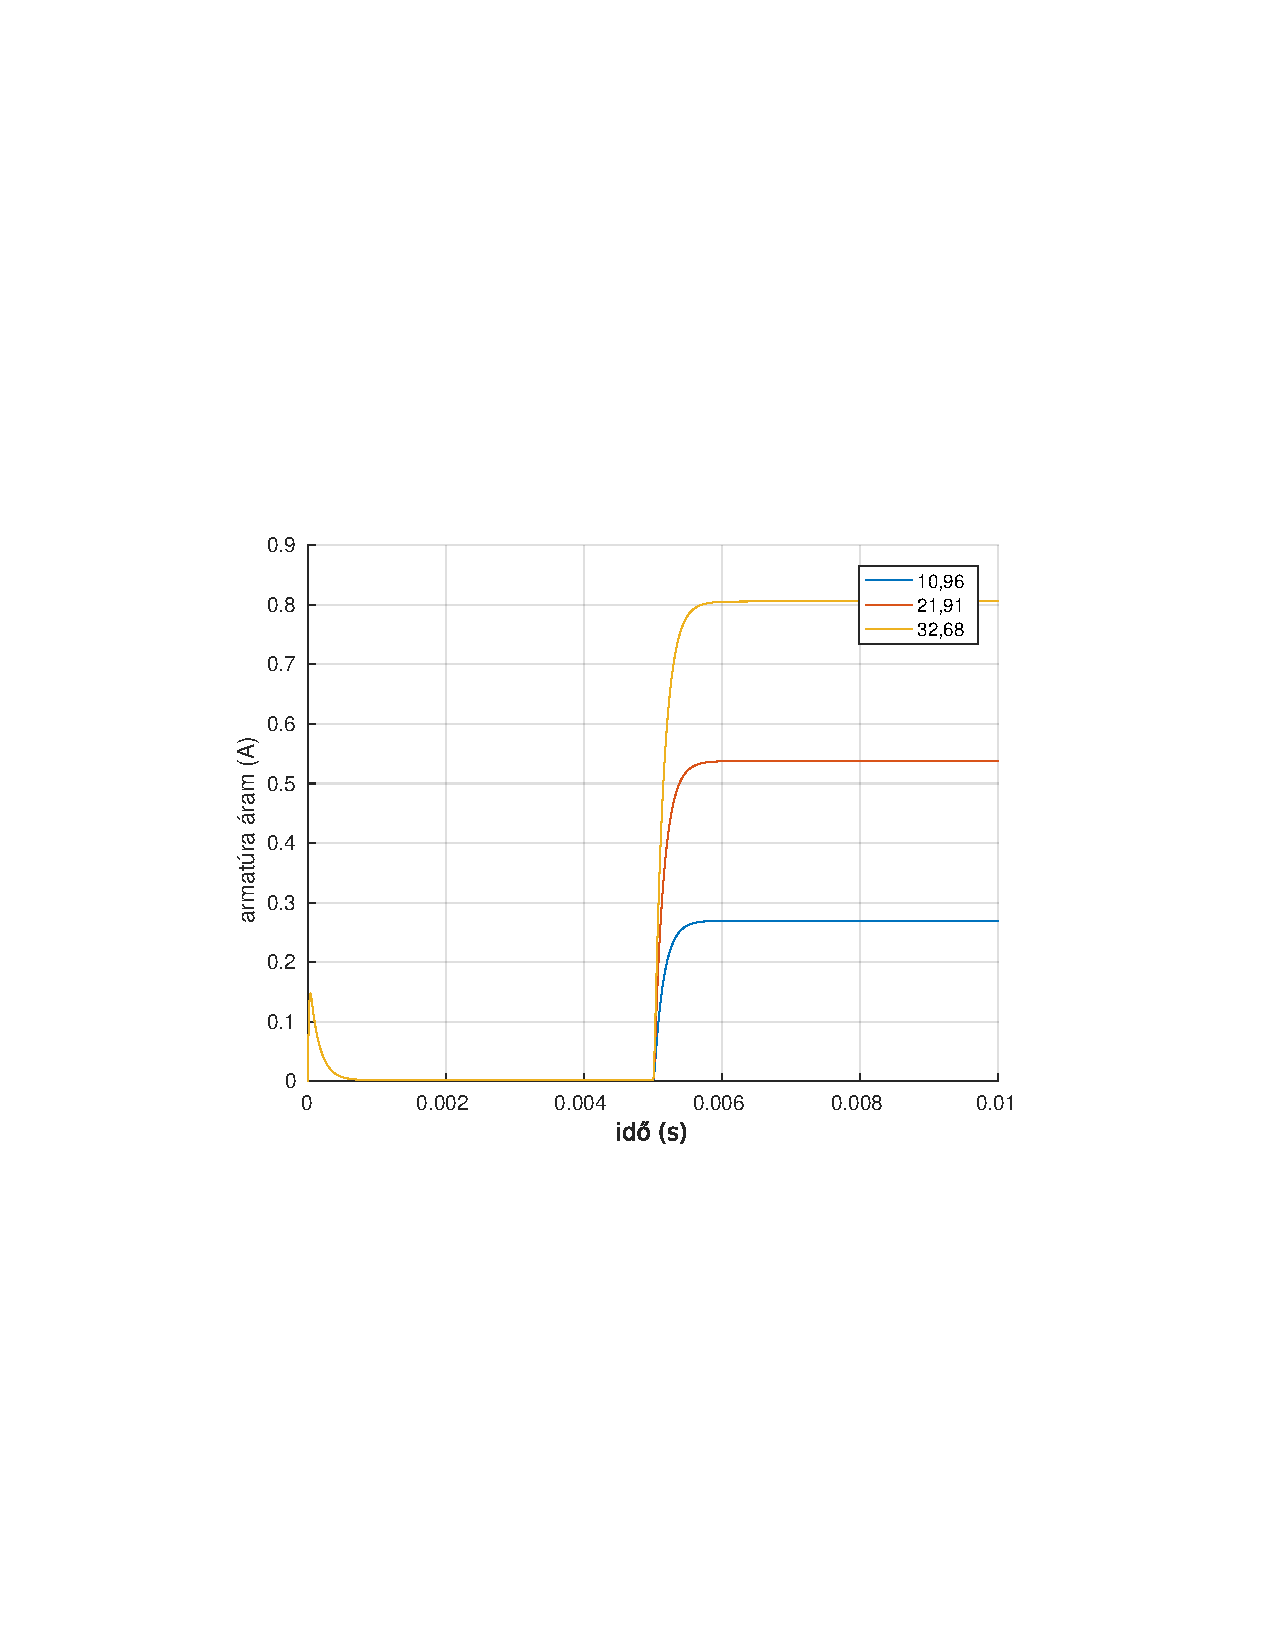
\includegraphics[width=\linewidth, trim=100 240 80 252, clip]{6-i}
		\caption{Áram válasz}
	\end{subfigure}
	\caption{Különböző amplitúdókra adott válasz}
	\label{fig:szorg2}
\end{figure}

A maximális terhelőnyomaték
\begin{equation}
	\tau_\text{t}^\text{max} = \pm0,0101\text{ Nm}
\end{equation}
